\documentclass[letterpaper, 11pt]{article}
%\usepackage[hmargin = 1in, vmargin = 1in]{geometry}
\usepackage{amsmath}
\usepackage{amssymb}
\usepackage{enumitem}
\usepackage{mathrsfs}
\usepackage{tikz}
\usepackage{graphicx}
\usepackage{algorithmicx}
\usepackage{algpseudocode}
\usepackage{hyperref}
\hypersetup{
    colorlinks=true,
    linkcolor=blue,
    filecolor=magenta,      
    urlcolor=blue,
}
% \doublespacing
\setlength{\headheight}{14pt}
\usepackage{fancyhdr}
\pagestyle{fancy}
\rhead{Gabriel Wallace}
\lhead{Comp Sci 3130}

\newcommand{\card}{\text{Card}}
\newcommand{\N}{\mathbb{N}}
\newcommand{\R}{\mathbb{R}}
\newcommand{\Z}{\mathbb{Z}}
\newcommand{\Q}{\mathbb{Q}}

\newcommand{\inv}{^{-1}}
\newcommand{\abs}[1]{\lvert #1 \rvert}
\newcommand{\hwnumber}[1]{\medskip \noindent\textbf{#1.} \smallskip}
\newcommand{\hwnumbersec}[3]{\medskip \noindent\textbf{#1.} Section #2 \##3 \smallskip}
\newcommand{\Mod}[1]{\ \mathrm{mod}\ #1}
\newcommand{\Alg}[1]{\medskip \noindent\textbf{ALGORITHM} \( #1 \)} 
\newcommand{\To}{\textbf{ to }}

\begin{document}
\section{Theoretical Analysis}
The theoretical analysis of all the sorting algorithms were covered in class.
For reference, we have the table of the relevant sorting algorithms and their
efficiency for the best, worst, and average cases. 

\begin{center}
\begin{tabular}{l | l l l}
  Algorithm & Best  & Worst  & Average  \\
  \hline
  Selection & \(\Theta(n^2)\) & \(\Theta(n^2)\) & \(\Theta(n^2)\) \\
  Insertion & \(\Theta(n)\) & \(\Theta(n^2)\) & \(\Theta(n^2)\) \\
  Bubble & \(\Theta(n^2)\) & \(\Theta(n^2)\) & \(\Theta(n^2)\) \\
  Bubble (with swaps) & \(\Theta(1)\) & \(\Theta(n^2)\) & \(\Theta(n^2)\) \\
  Quick & \(\Theta(n \log n)\) & \(\Theta(n^2)\) & \(\Theta(n\log n)\) \\
  Merge & \(\Theta(n \log n)\) & \(\Theta(n\log n)\) & \(\Theta(n\log n)\) \\
\end{tabular}
\end{center}

\section{Empirical Analysis}
The following section covers the empirical analysis of the above sorting
algorithms. Due to memory issues (for more details see ), quicksort gets its
own section. All the algorithms were implemented in Python, and the source code
can be found on
\href{https://github.com/gwallace04/cs3130/blob/master/projects/proj2/proj2.py}
{GitHub}. The tables with the raw data for the analysis can be found in section
BLANK.

\subsection{Graphs and Discussion}
We have the graphs from all the algorithms below.
\begin{figure}[h]
  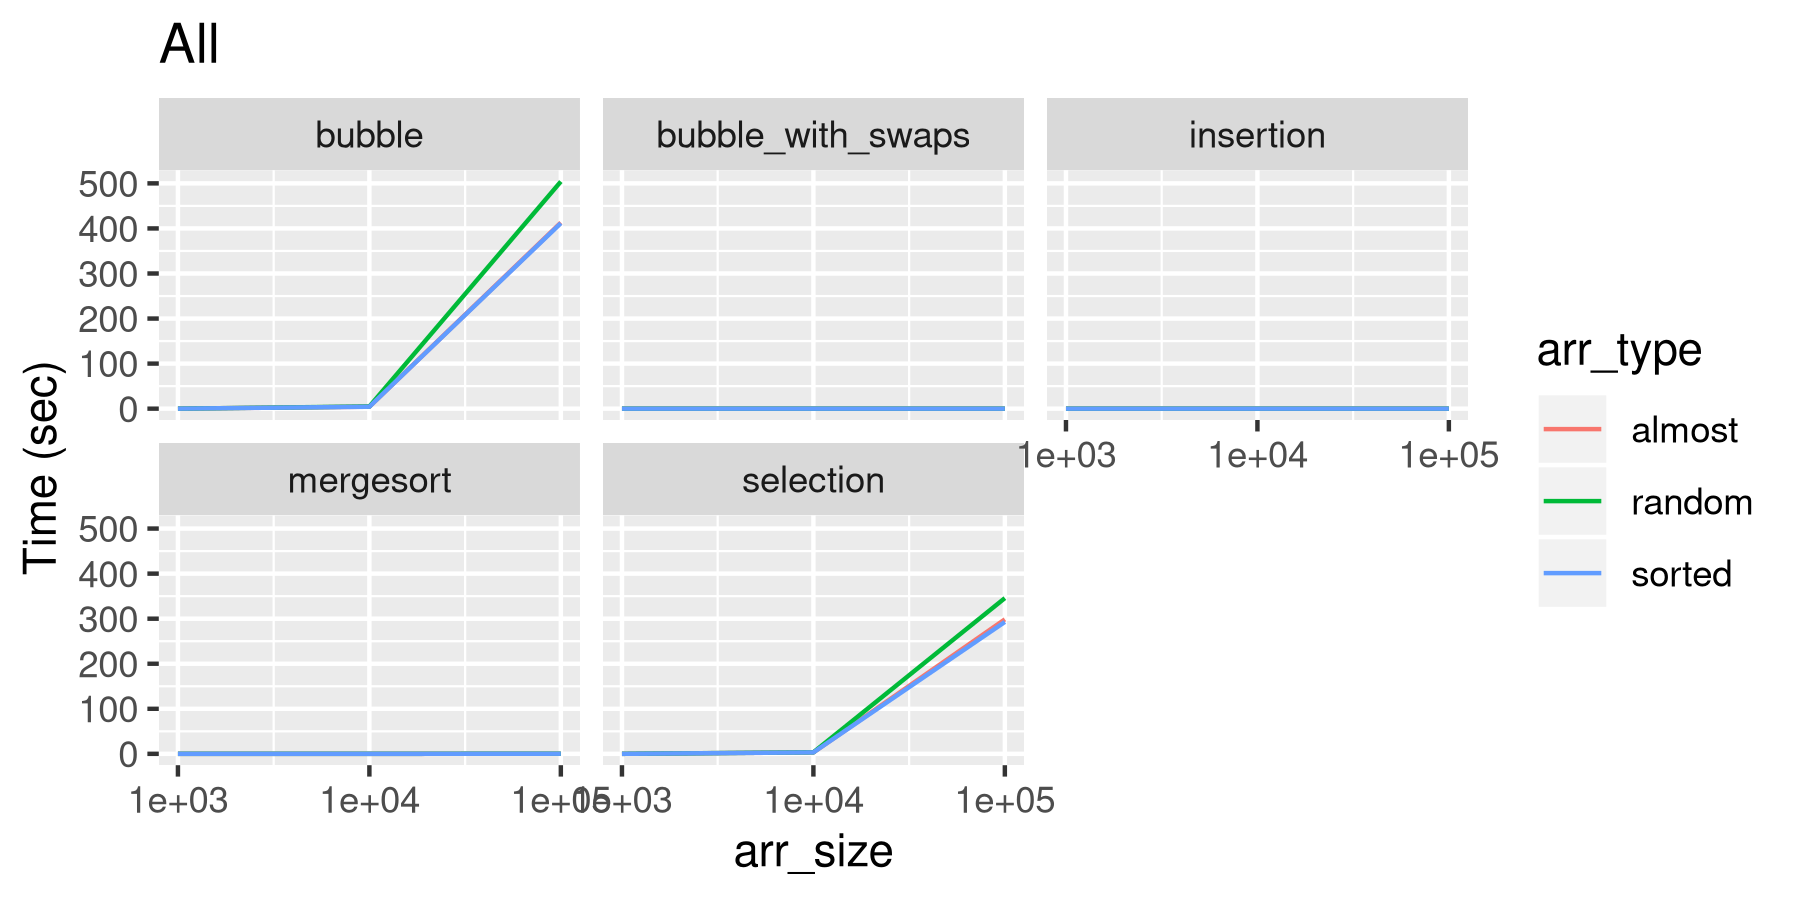
\includegraphics[width=\linewidth]{all.png}
\end{figure}

From the graphs we can see that bubble and selection sort grow much
quicker than the other sorting algorithms. So much so, that the scale of the
vertical axis makes it to where the other algorithms are basically a flat line.
To see the growth more clearly of the other sorting algorithms, we have separate
graphs. 

\begin{figure}[ht]
  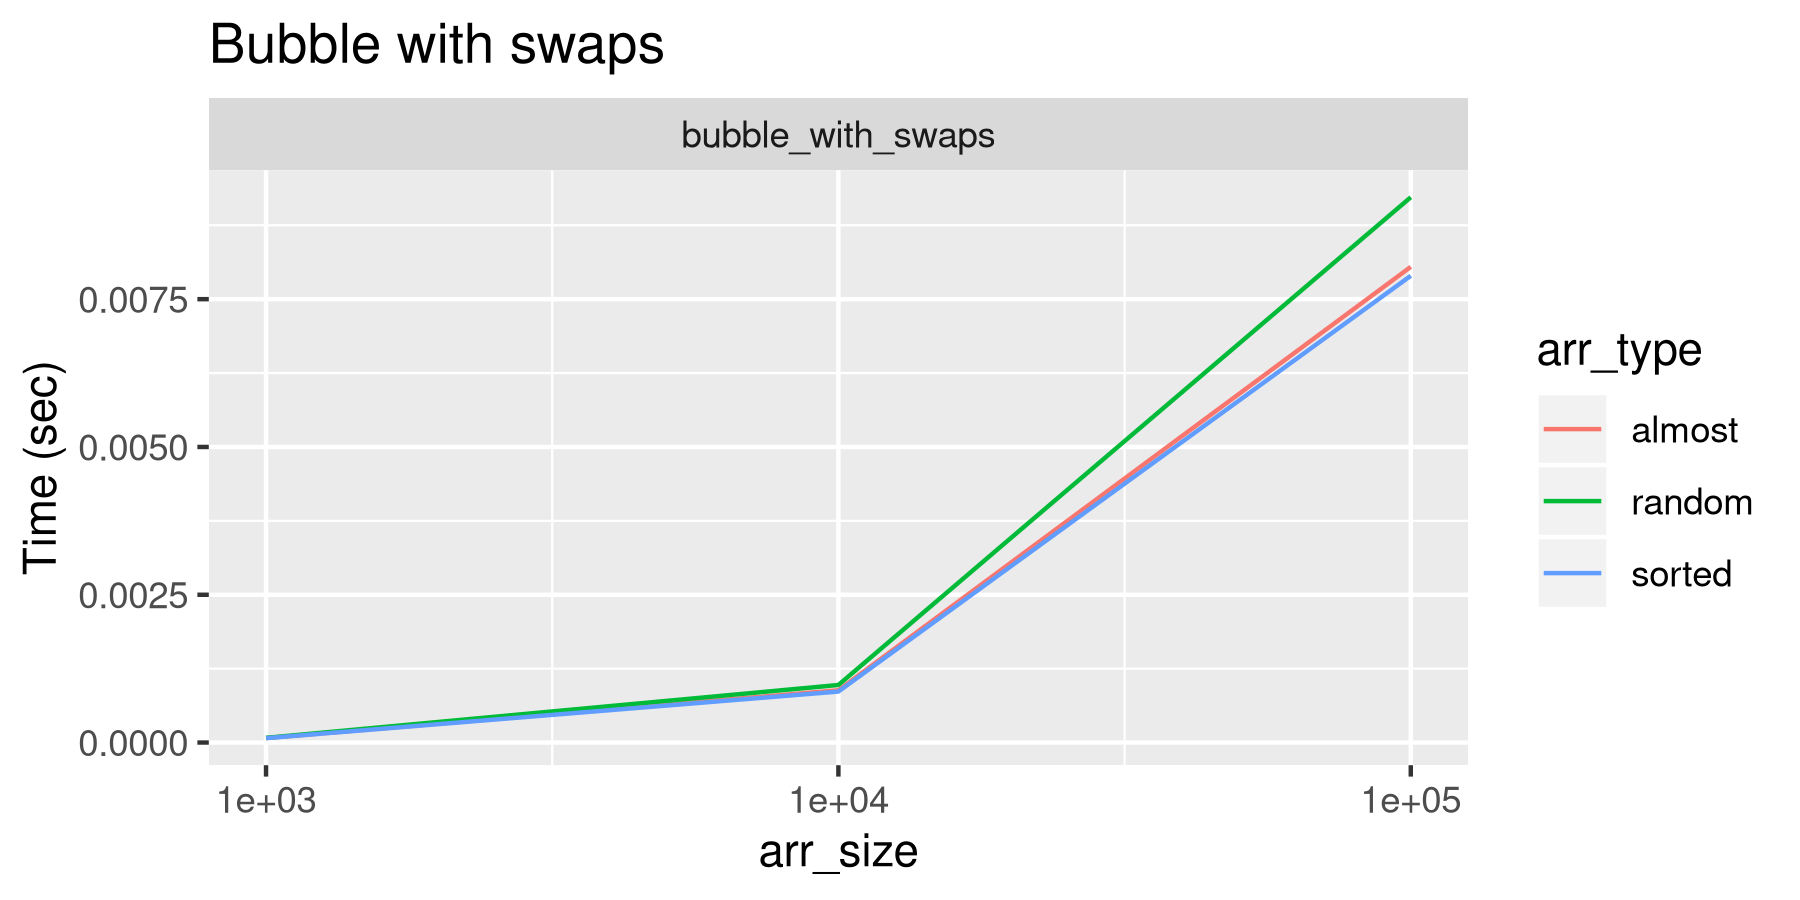
\includegraphics[width=\linewidth]{bubble_with_swaps.png}
\end{figure}

\begin{figure}[ht]
  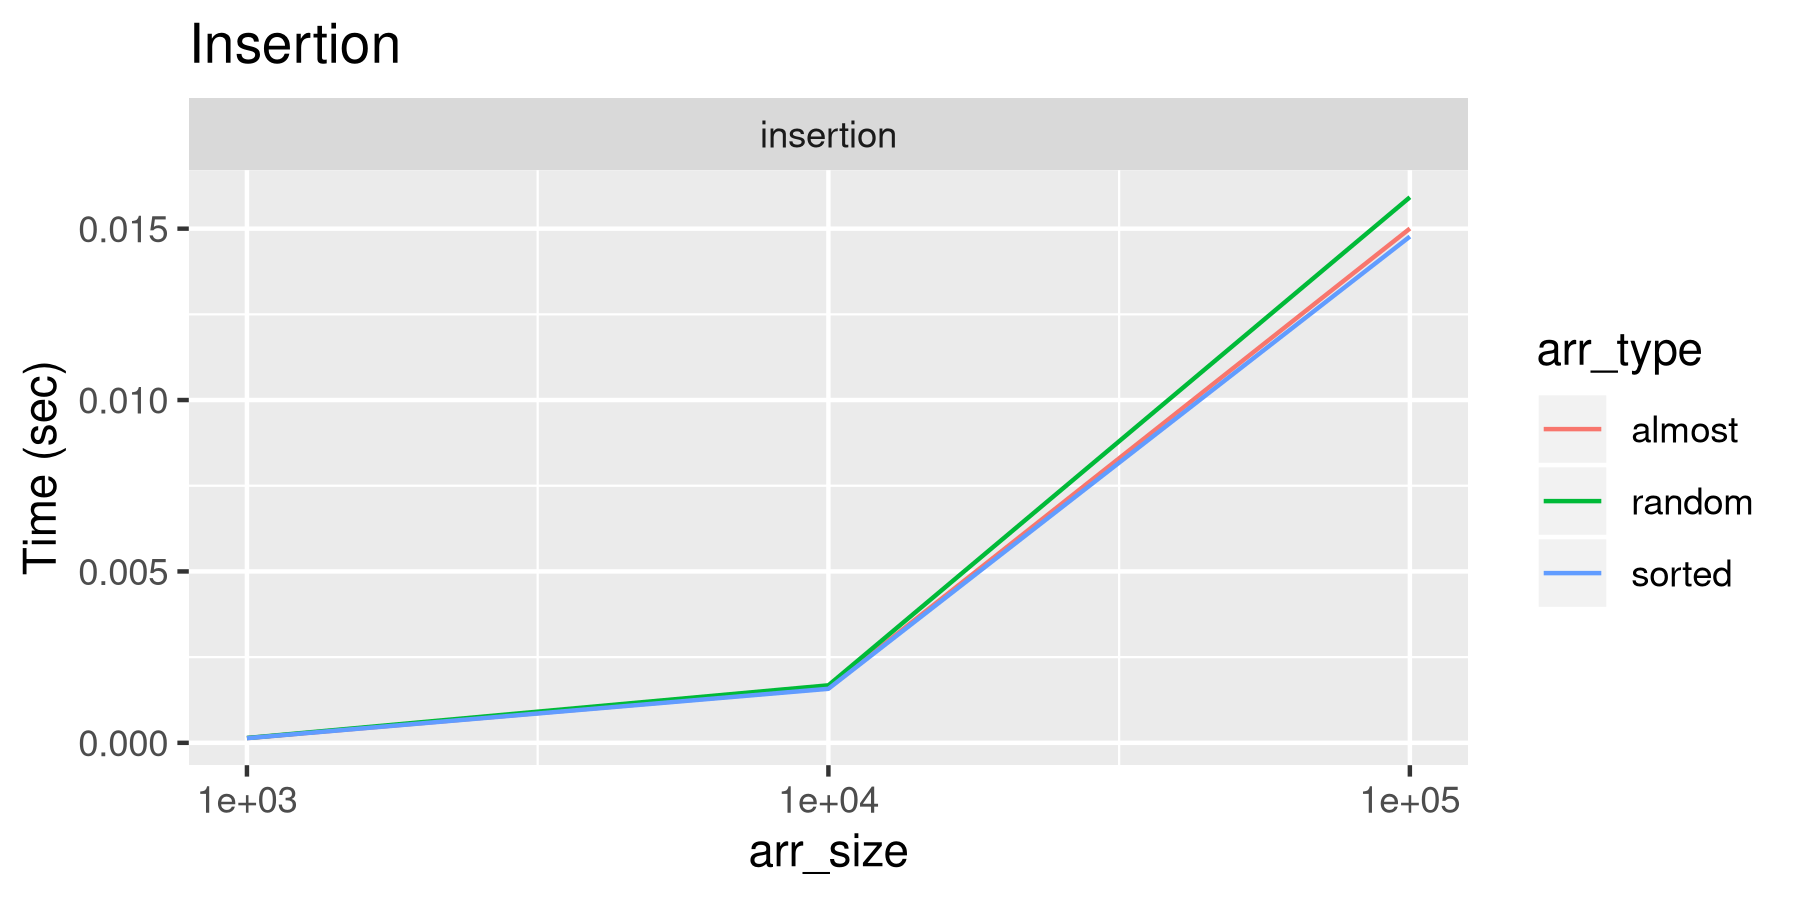
\includegraphics[width=\linewidth]{insertion.png}
\end{figure}

\begin{figure}[t]
  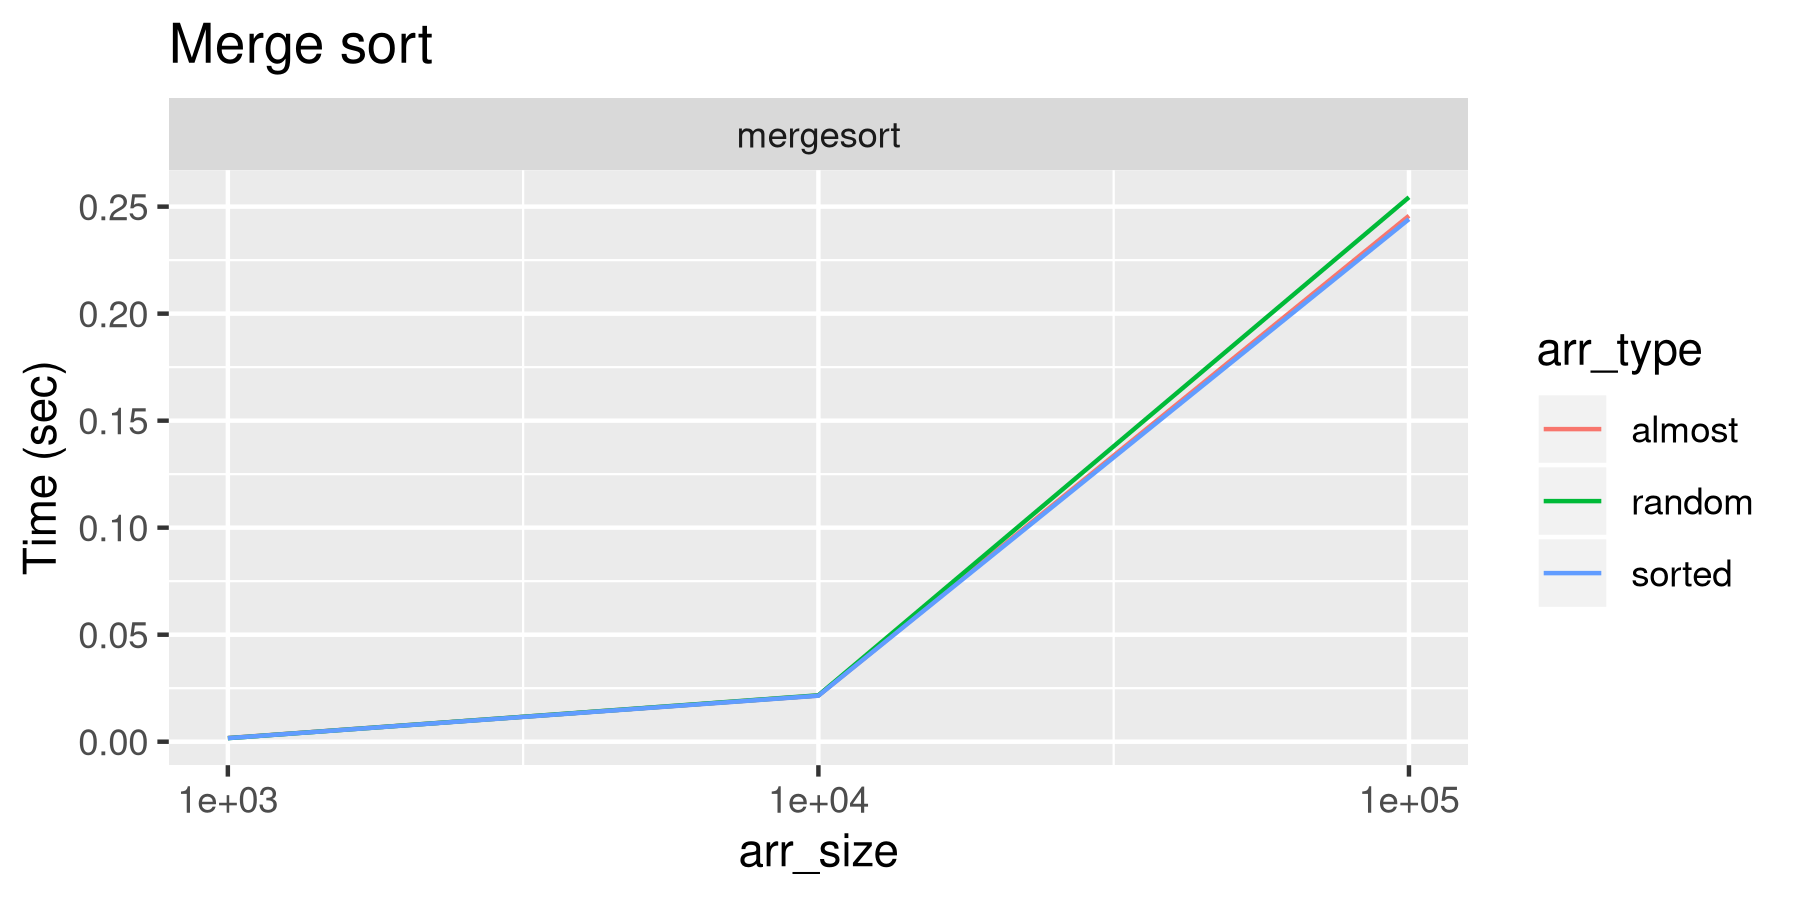
\includegraphics[width=\linewidth]{mergesort.png}
\end{figure}


It is hard to tell with only three data points, but we can see that all the
sorting algorithms have similar shapes, albeit with bubble and selection having
much steeper curves. This makes sense for the most part since most of the
algorithms (except for mergesort), have efficiency \(\Theta(n^2)\). From a
purely theoretical view, we would expect to see that mergesort has a less steep
curve than the other algorithms since it is non-adaptive and has efficiency
\(\Theta(n \log n)\). However, the curve is the same and, in fact, the absolute
time is much higher than either the improved bubble sort or the insertion sort.
On the other hand, our theoretical analysis is supported by the data for
mergesort being non-adaptive because the curves for all the array types
(sorted, almost sorted, and random) are essentially the same. This does not
hold for all the algorithms that are adaptive.  

In tables \ref{table:almost} and \ref{table:random}, we can see that the
improved bubble sort performs the best for almost sorted and random arrays
respectively. Insertion sort is a close second. This hold true for sorted lists
as well, which confirms our theoretical analysis with the improved bubble sort
having best case efficiency \(\Theta(1)\). Of course, the question of which
sorting algorithm performs best on an already sorted list is a bit moot.  

Selection and regular bubble sort perform much worse than the others. This
shows that even if two algorithms have the same order of growth, this does not
necessarily mean they are as fast as one another. 

\begin{table}[h]
\centering
  \begin{tabular}{l c}
    Algorithm & Average time (sec) \\
    \hline
    Bubble with swaps &  0.00300\\
    Insertion        &   0.00558\\
    Mergesort       &    0.0897\\
    Selection      &  101\\
    Bubble         &  139\\
  \end{tabular}
  \caption{Almost sorted}
  \label{table:almost}
\end{table}

\begin{table}[h]
\centering
  \begin{tabular}{l c}
    Algorithm & Average time (sec) \\
    \hline
		Bubble with swaps   & 0.00300\\
		Insertion           & 0.00558\\
		Mergesort           & 0.0897 \\
		Selection           & 101\\
		Bubble              & 139\\
  \end{tabular}
  \caption{Random}
  \label{table:random}
\end{table}

\subsection{Quicksort}
The space efficiency of quicksort is \(\Theta(n)\). Therefore, in our code,
when we try to apply quicksort to an already sorted array (the worst case
scenario), we quickly hit Python's recursion stack limit of 1000. This is true
even for random arrays bigger than around a 1000. Thus, quicksort was not
included with the other algorithms. We did, however, run quicksort on arrays of
random elements to confirm our theoretical analysis. The plot of the analysis
can be found in figure \ref{fig:quick}. 

\begin{figure}[h]
  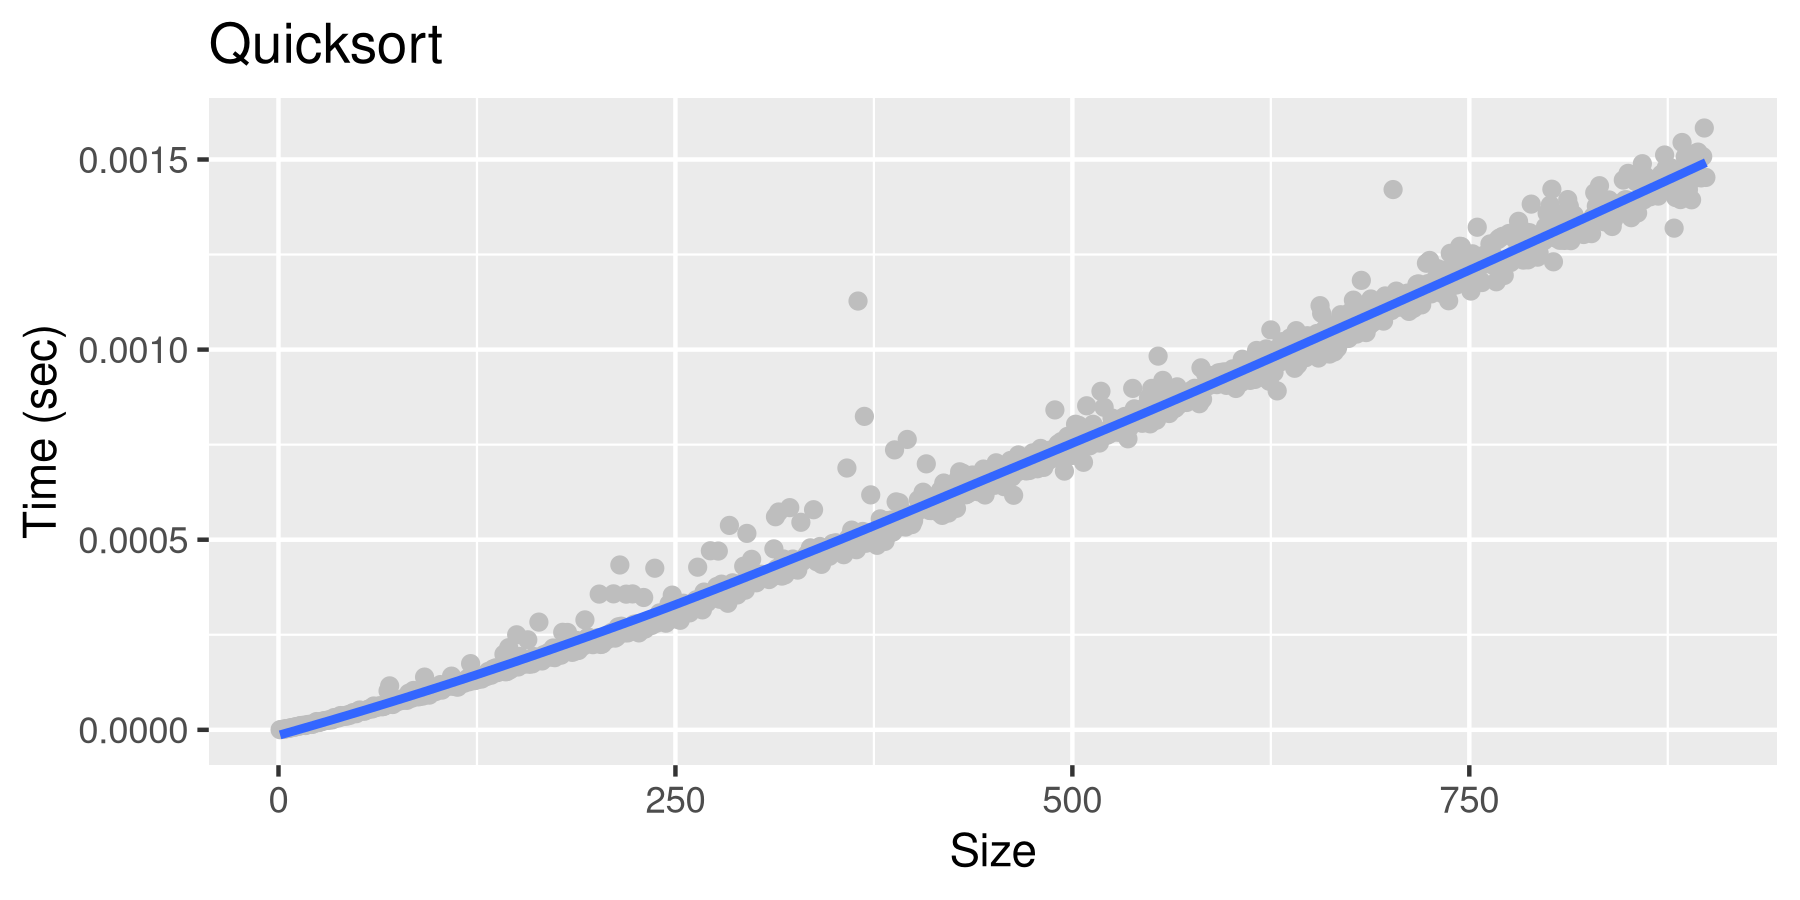
\includegraphics[width=\linewidth]{quick.png}
  \label{fig:quick}
\end{figure}

From this plot, we can see that our empirical analysis supports our theoretical
analysis that quicksort is of efficiency \(\Theta(n \log n)\). 

\appendix
\section{Tables of Raw Data}
Test

\end{document}
